\documentclass[12pt, a4paper, twoside]{book}
\usepackage{import}
\subimport{../}{preamble}
\begin{document}

\chapter{Fast Spectroscopy of Plasmonic Dimer Make/Break Junctions}

One of the aspects of the microscope platform not discussed in the main text is the capability for fast spectroscopy with down to \SI{10}{\micro\second} resolution. This was developed in order to measure the initial contact dynamics of plasmonic tip dimers as they come into conductive contact, along with the plasmonics of  break junctions formed between the two Au surfaces in a touching tip dimer. Mechanically controllable break junctions (MCBJs) similar to the Au contact formed between tips are well documented and have formed the basis of quantised conductance studies in 3D systems at room temperature (as opposed to the original 2DEG systems) \cite{armstrong2010channel, costa1997conductance, costa1997conductance2, costa1997conductance3, landman1996reversible, natelson2012mechanical, rodrigues2000signature, rodrigues2002quantum, sabater2012mechanical, sorensen1998mechanical, yanson2005atomic}.

\FloatBarrier
\section{Experimental Setup}

\begin{figure}[bt]
\centering
\fontsize{10pt}{1em}\selectfont
\def\svgwidth{0.69\textwidth}
\subimport{./figures/}{fast_setup.pdf_tex}
\caption[Diagram of the fast spectroscopy setup]{\textbf{Diagram of the fast spectroscopy setup.} The setup consists of a custom shutter, built from a disassembled hard drive, and a monochromator-CCD pair. Kinetics acquisition on the CCD, along with the shutter mechanism, is triggered by fast electrical signals from the tips which are measured on the oscilloscope.}
\label{fig:fast_setup}
\end{figure}

\begin{figure}[bt]
\begin{tikzpicture}
\node [below left] at (0,0) {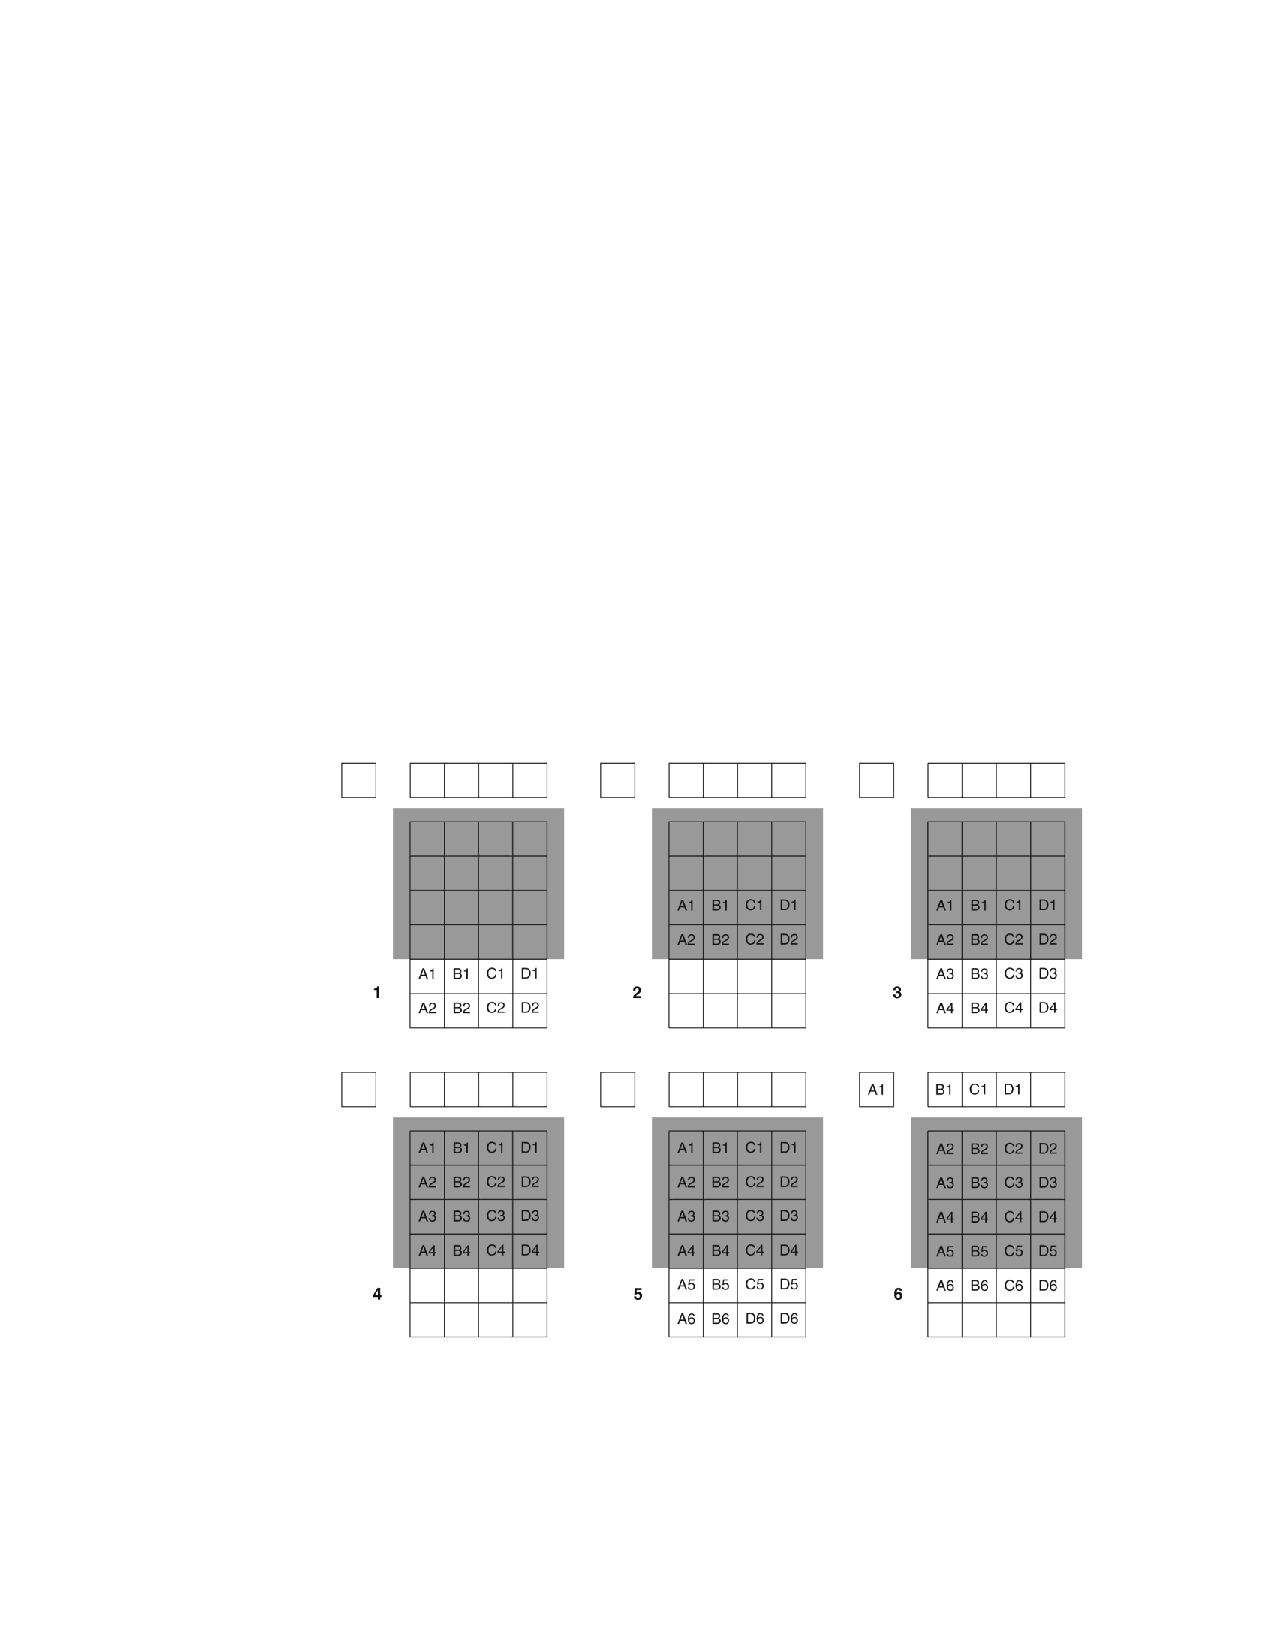
\includegraphics[width=0.39\textwidth]{figures/kinetics_diagram_1}};
\node [below right] at (0,0) {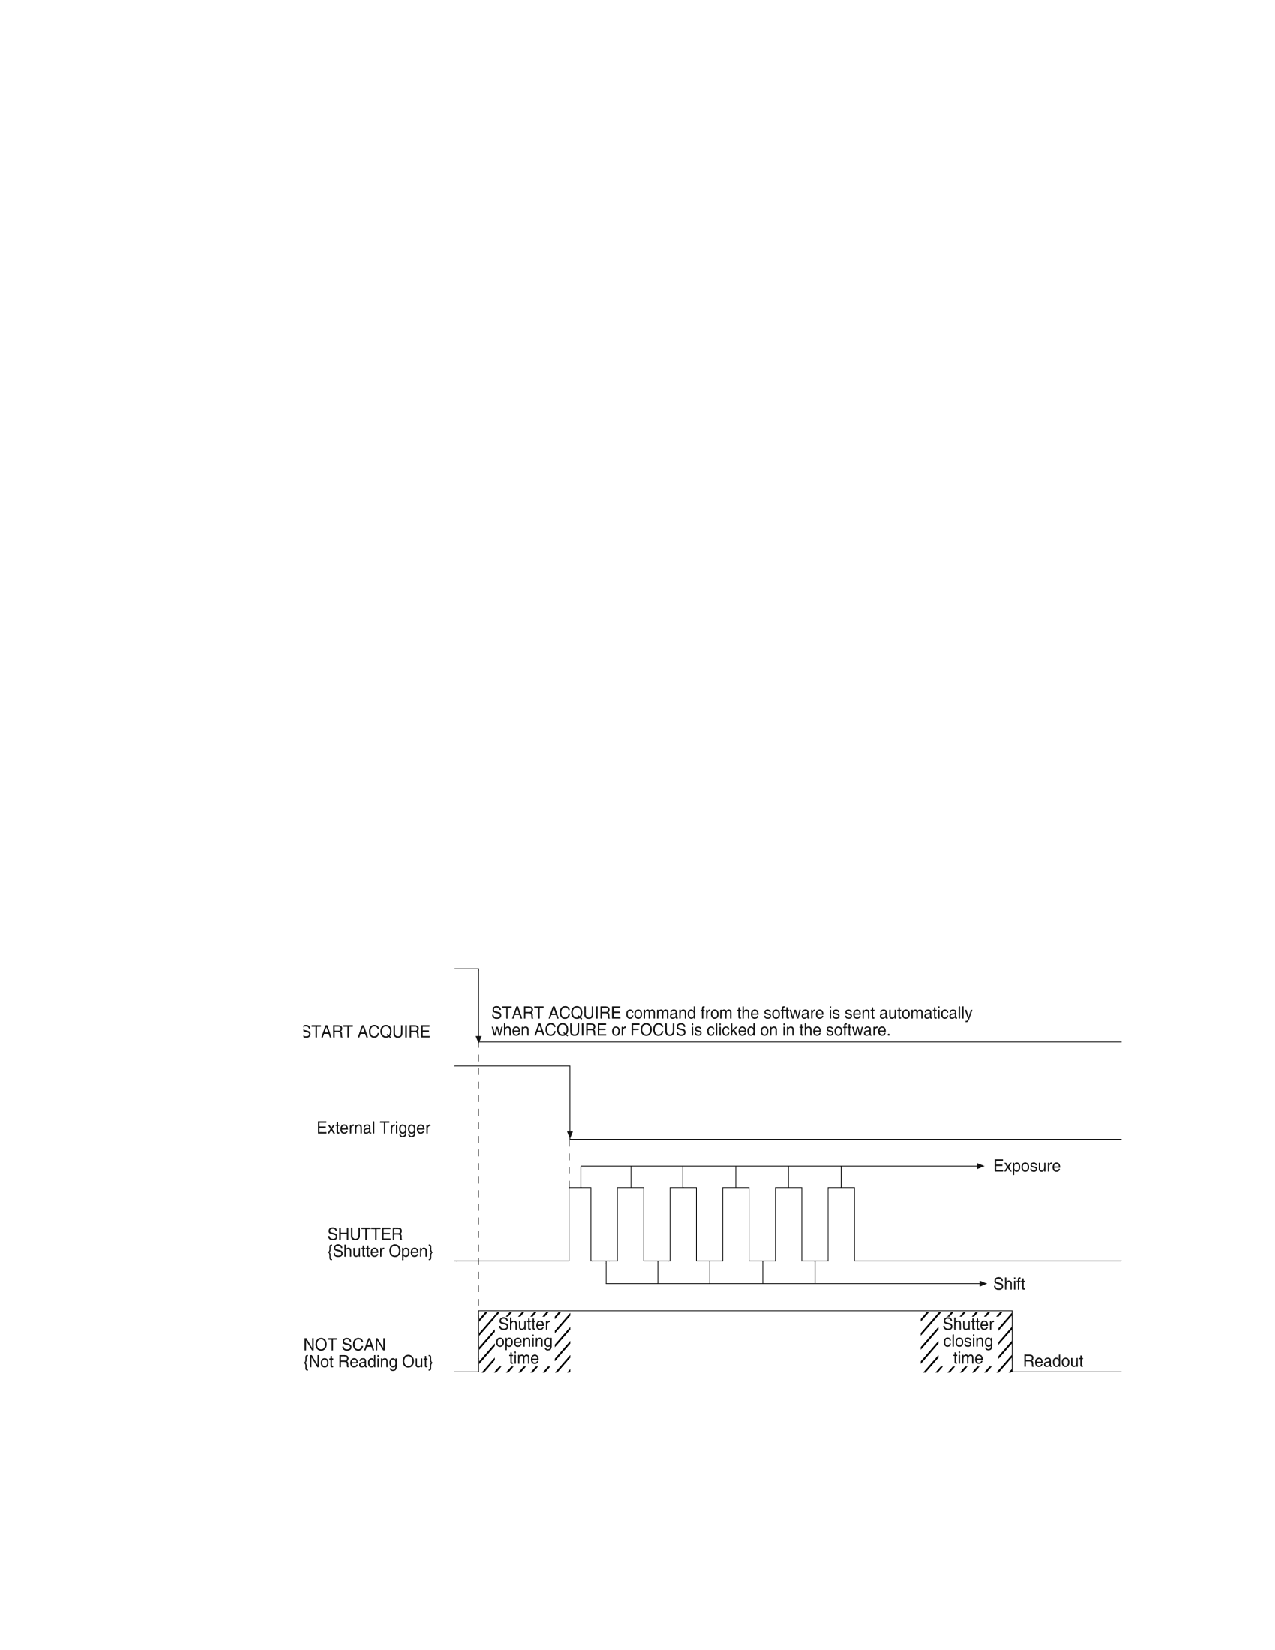
\includegraphics[width=0.59\textwidth]{figures/kinetics_diagram_2}};
\end{tikzpicture}
\caption[Diagram showing kinetics mode acquisition on the CCD]{\textbf{Diagram showing kinetics mode acquisition on the CCD.} An exposed region of the CCD is shuffled into a mechanically or optically masked region. Once the whole CCD has been exposed the image is read out. This acquisition process, along with the opening of the fast shutter, is triggered by an external TTL pulse from an oscilloscope. These images are taken from the Princeton Instruments PIXIS CCD manual.}
\label{fig:kinetics_diagram}
\end{figure}

The experimental setup for fast spectroscopy is shown in \autoref{fig:fast_setup}. Collimated scattered light from the tips is focussed down onto the end of the shutter blade and then, with the shutter open, reimaged onto the entrance slit of a monochromator (Horiba Yvon Jobin Triax 320). The monochromator is paired with a CCD supporting a kinetics readout mode (Princeton Instruments PIXIS 256E), wherein charge is shuffled down the active CCD area after the single top-most line of pixels is exposed to produce a time-series of spectra. The time interval recorded during time-resolved spectroscopy is given by,
\begin{equation} t_{\mathrm{range}} = 256 (t_{\mathrm{exposure}} + t_{\mathrm{shift}}), \end{equation}
where $t_{\mathrm{exposure}}$ is the exposure period of each row of pixels and $t_{\mathrm{shift}}$ is the time taken to shift all pixels by one row. The shuffle speed is fast (\SI{9.2}{\micro\second}) compared with the readout time meaning it is possible to obtain resolutions around \SI{10}{\micro\second} with the complete image readout only once the kinetics process has completed. Kinetics acquisition is therefore good for measuring short-lived, single-shot events, similar in application to a streak camera. A coarse, \SI{150}{lines.mm^{-1}} diffraction grating is chosen to disperse the visible spectrum along the top row of the CCD. The fast spectroscopy path from its initial split off point at the beamsplitter is completely tubed to reduce any background noise incident on the sensitive CCD, with an opening only to place the shutter in the beam.

\begin{figure}[bt]
\centering
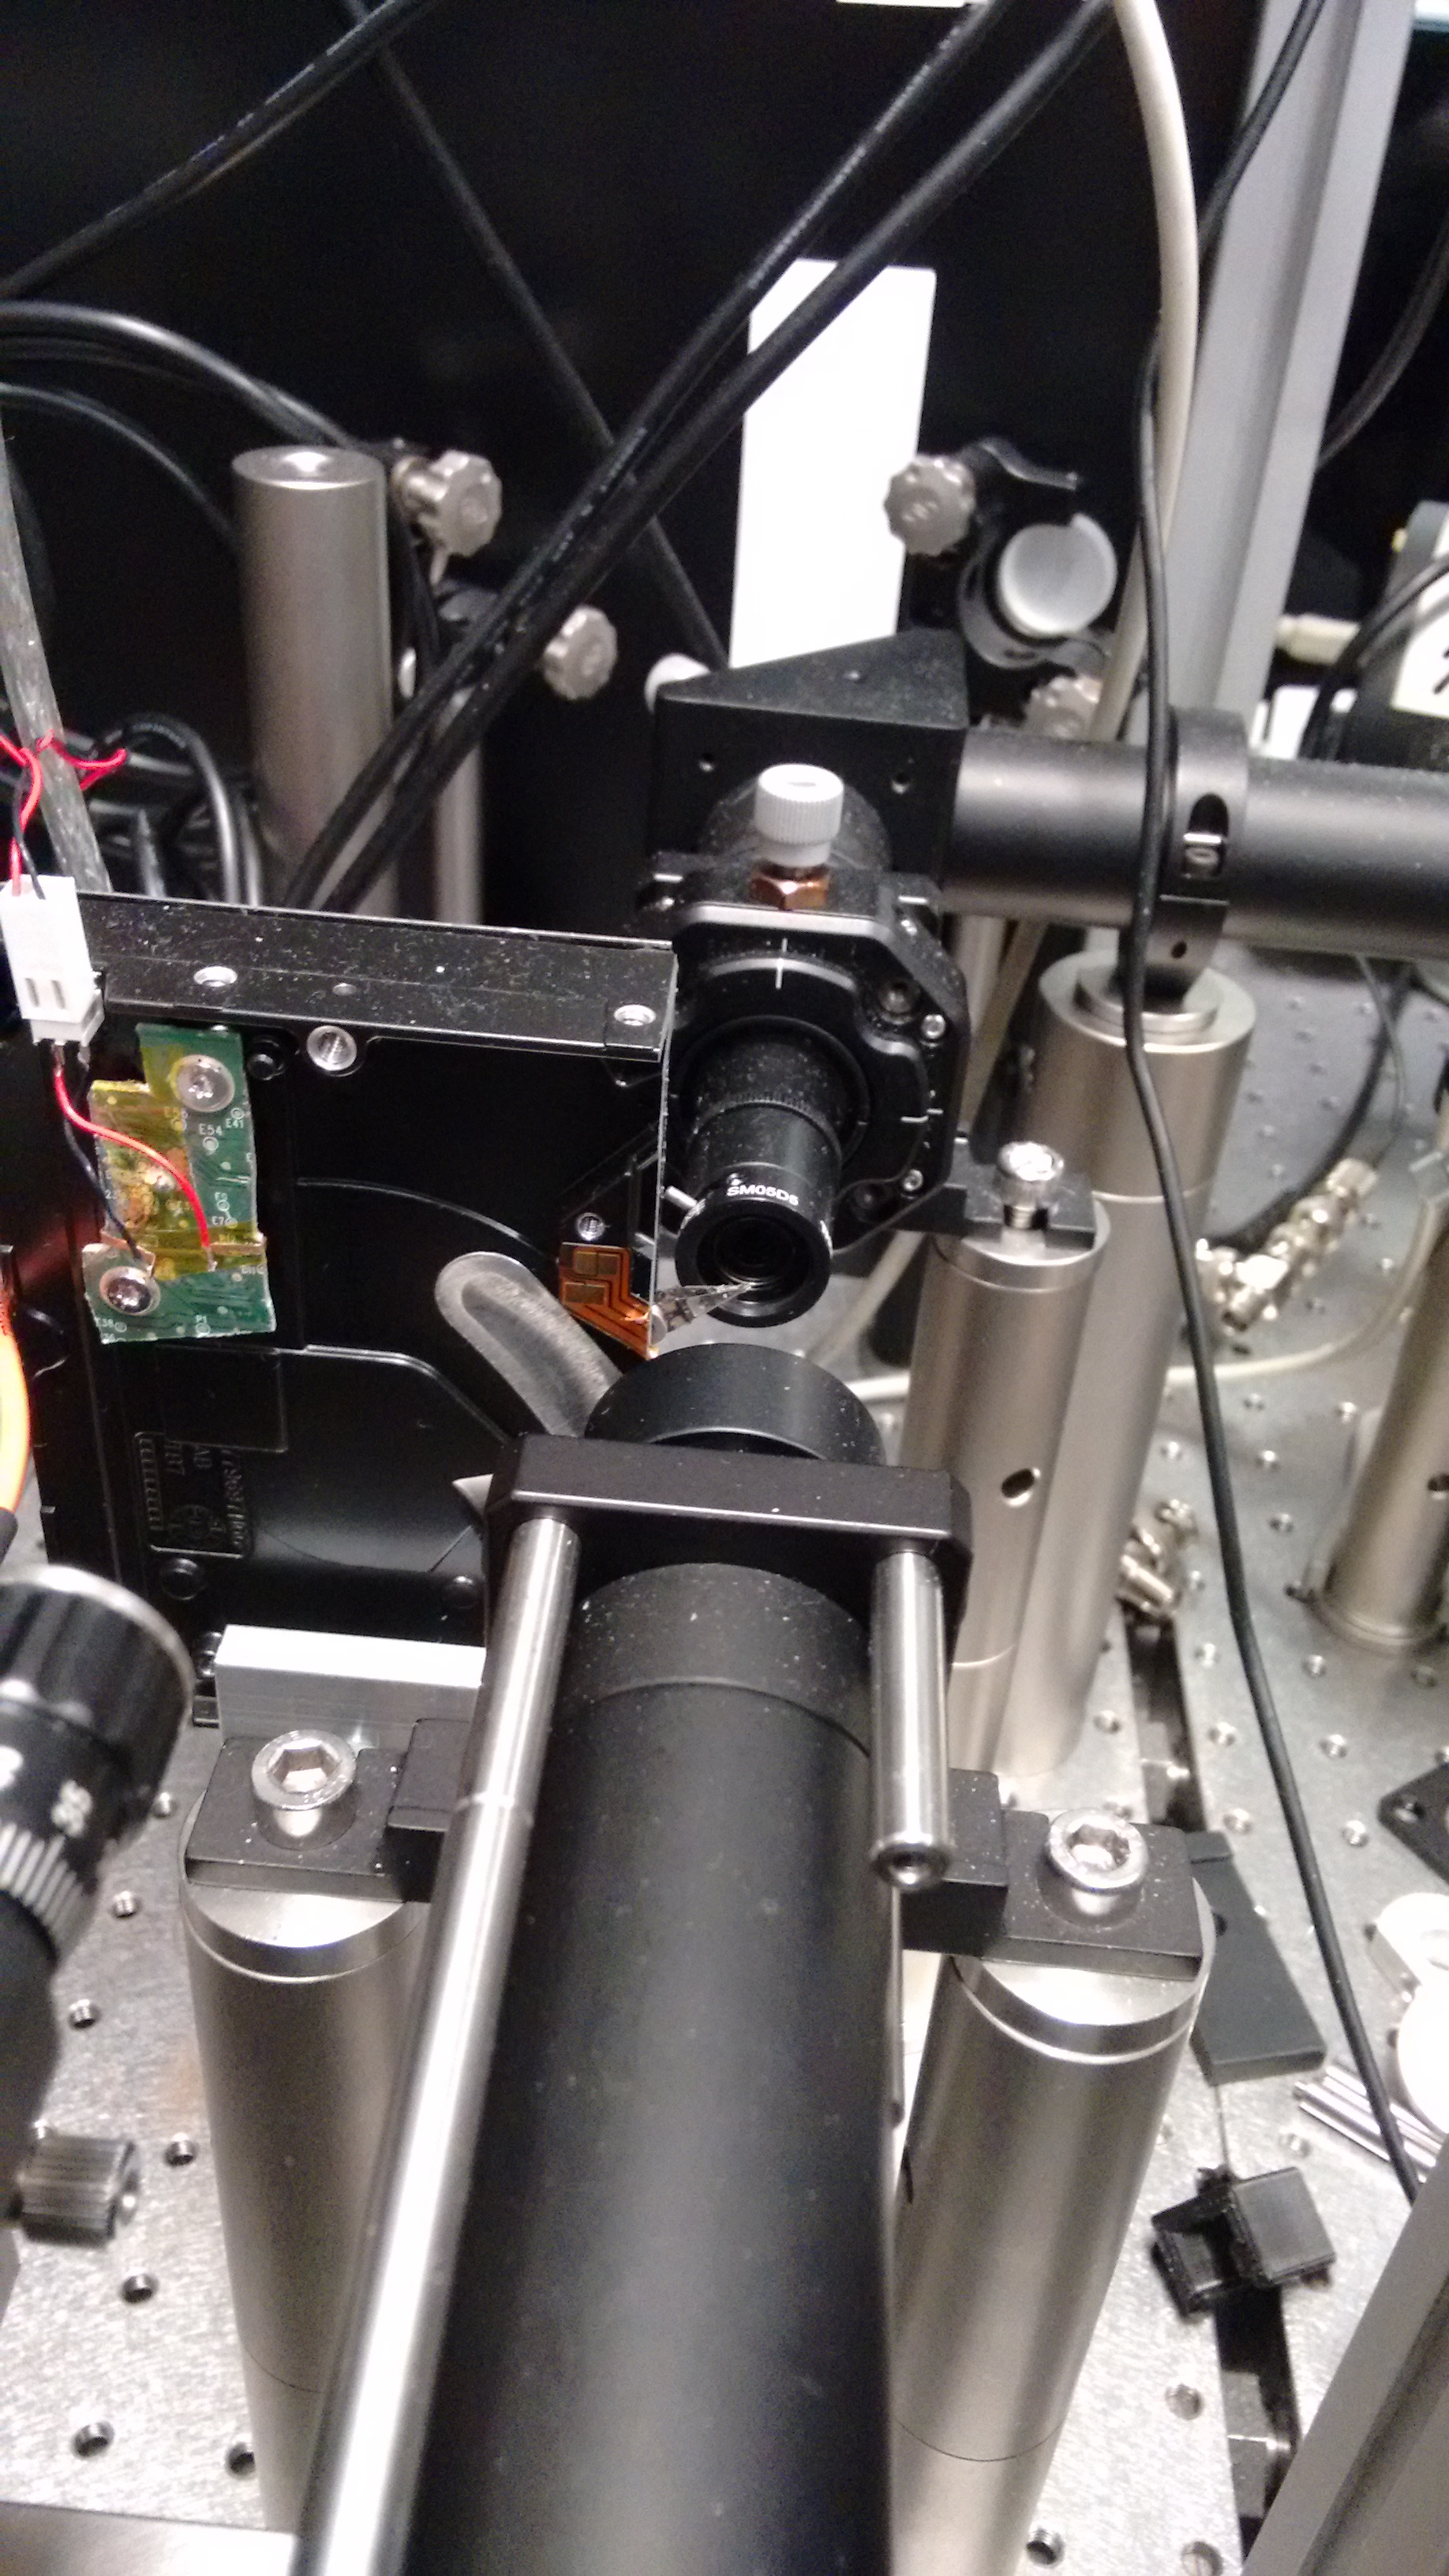
\includegraphics[width=0.45\textwidth, clip=true, trim=0 1300 500 900]{figures/hard_drive_shutter_1}
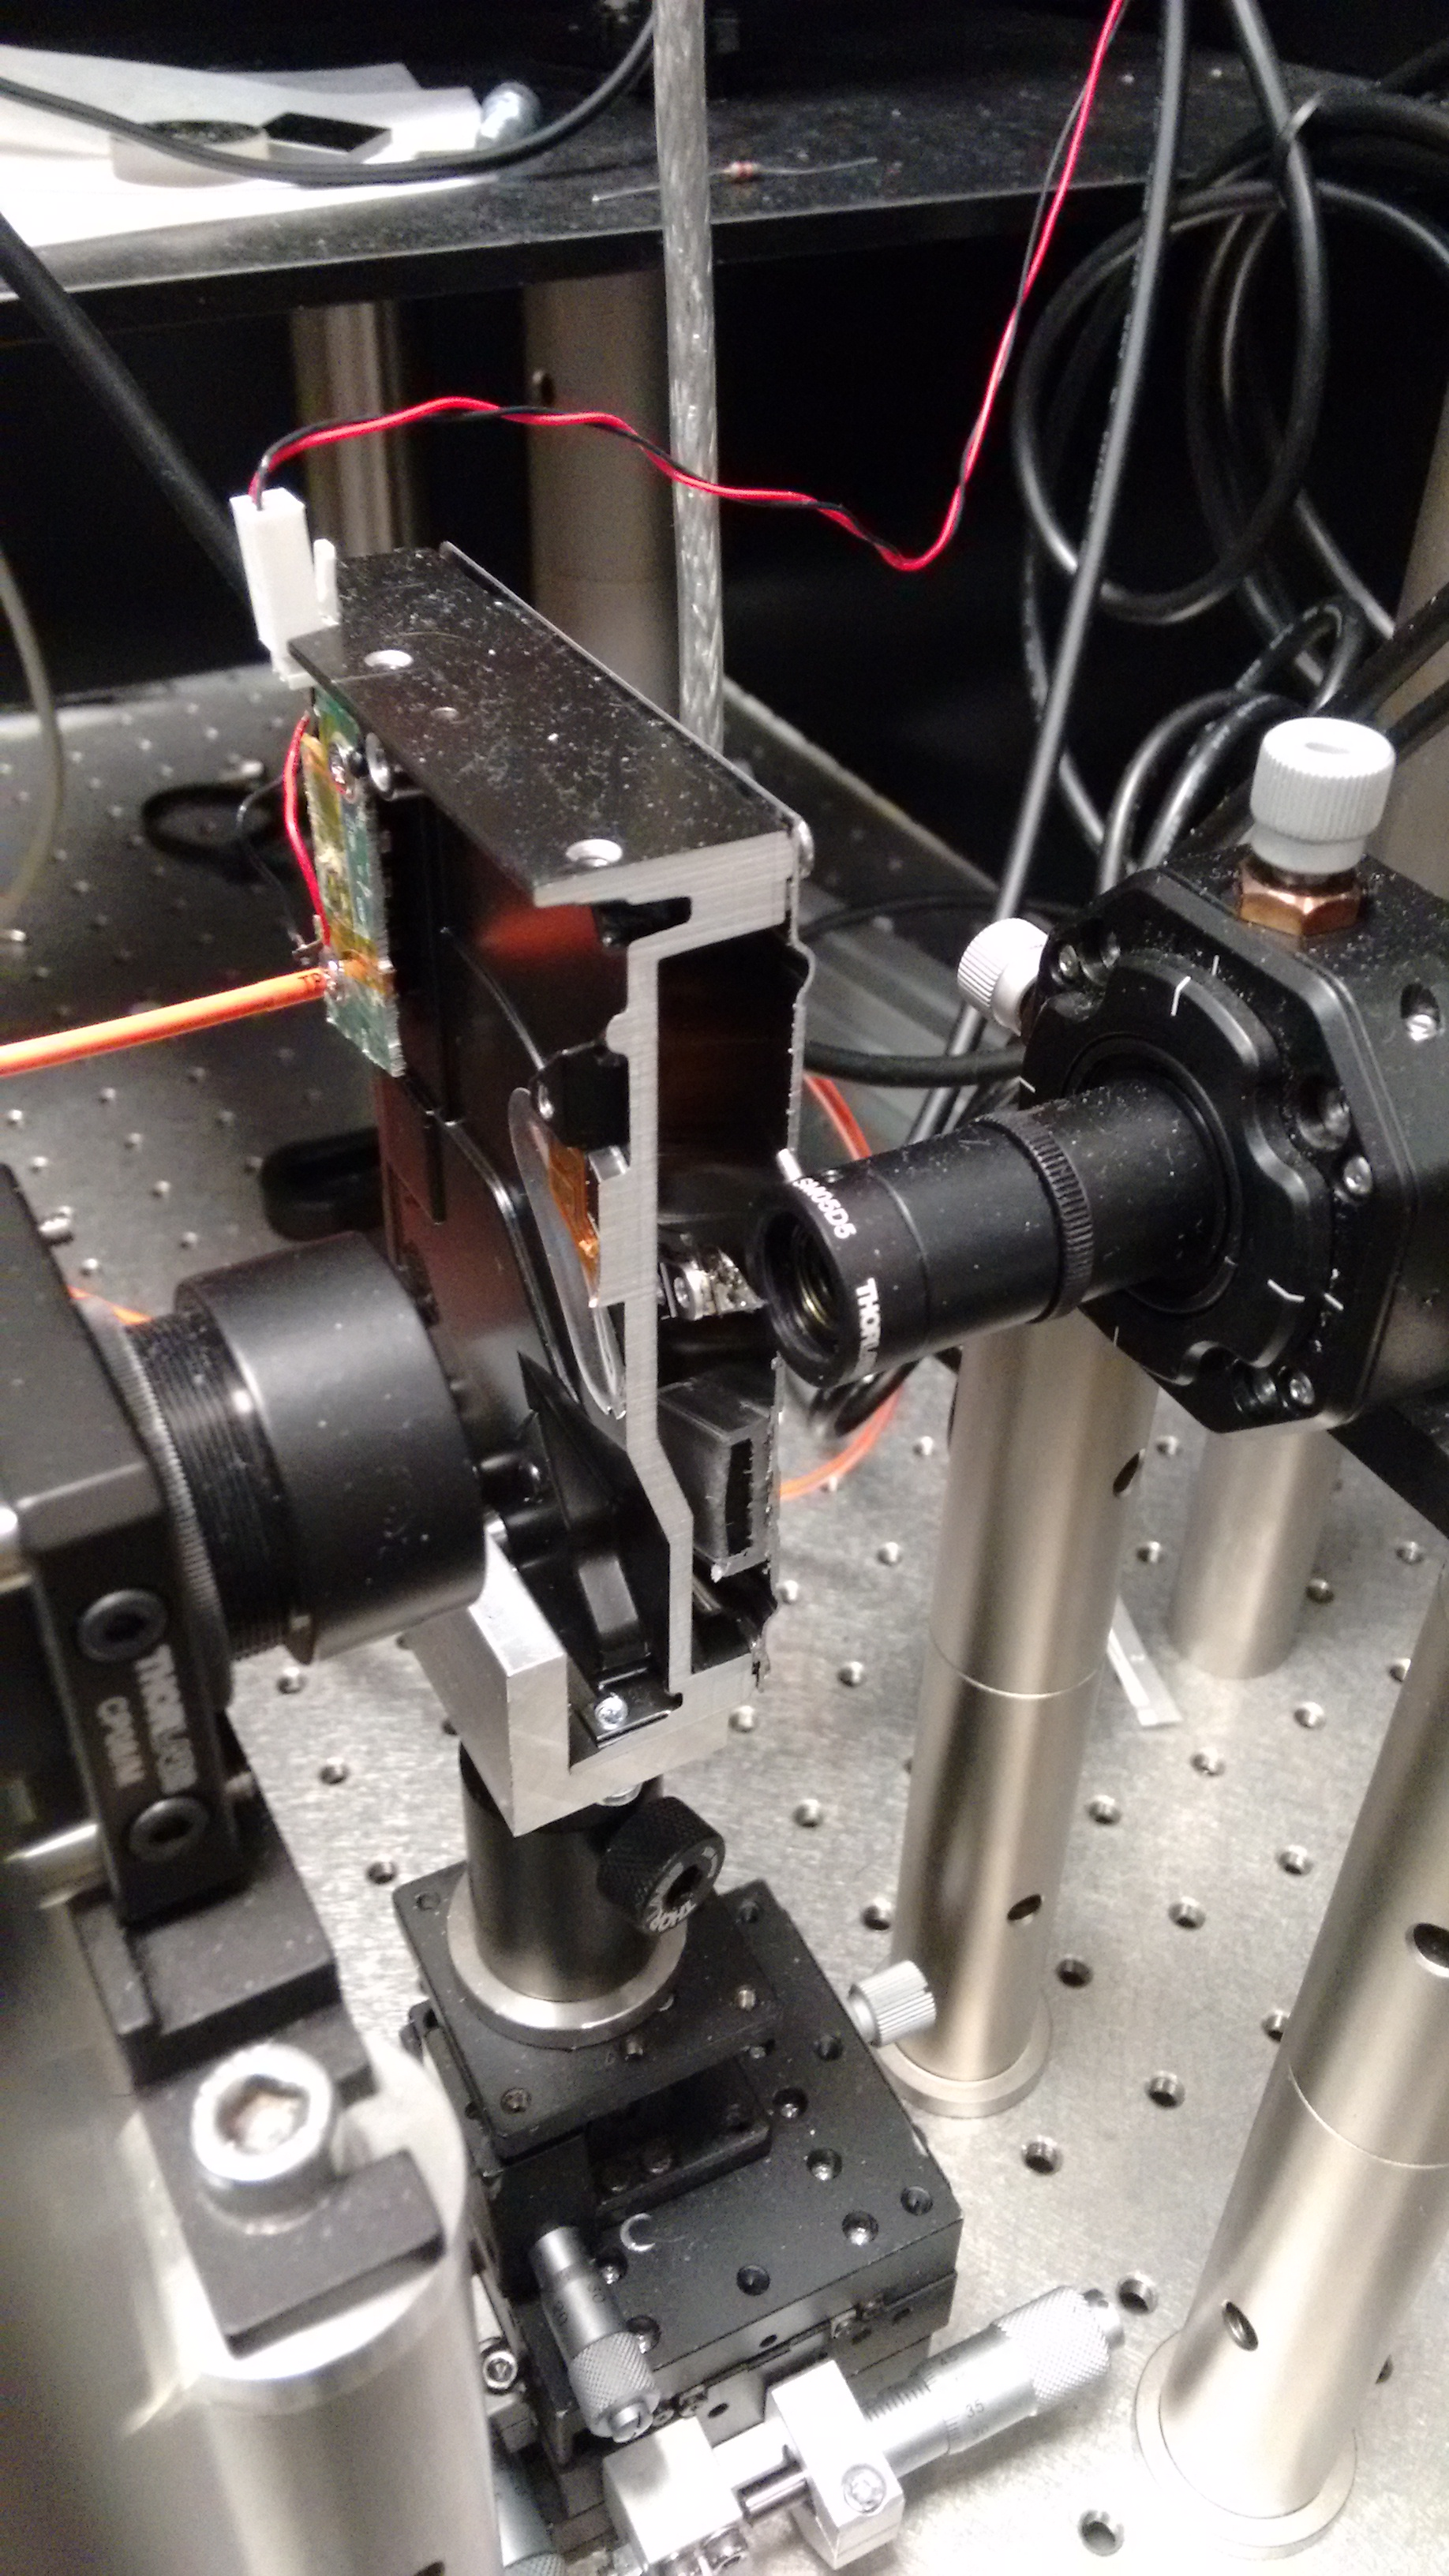
\includegraphics[width=0.45\textwidth, clip=true, trim=0 1000 0 800]{figures/hard_drive_shutter_2}
\caption[Images of the hard drive shutter]{\textbf{Images of the hard drive shutter.} The shutter works by passing a current through the hard drive voice coil, generating a magnetic field which quickly moves the read head via a Lorentz force. This functions as a shutter blade. The shutter blade is placed in the focus between two lenses in order to uncover the focussed beam spot in the shortest possible time. Rise times in this configuration are around \SI{300}{\micro\second}.}
\label{fig:hard_drive_shutter}
\end{figure}

The kinetics sequence is armed at the start of each experiment, waiting for a trigger signal to begin acquisition. Non-essential CCD procedures, such as continuous cleaning, are deactivated to improve the activation time upon receiving the trigger signal. The CCD is protected from pre-sequence overexposure by a custom-built fast shutter, constructed using the read head from a disassembled 3.5" computer hard-drive, shown in \autoref{fig:hard_drive_shutter}. The hard drive is mounted onto a 3D translation stage and the shutter blade is aligned in the focus of the scattered light such that the time taken to uncover the beam is minimised. Regular shutters are limited to \SI{8}{ms} opening times due to solenoid delay and thus the majority of a short, $\sim$\SI{10}{ms} make/break junction event would be missed. Use of the hard-drive voice coil mechanism enables shutter open times of around \SI{300}{\micro\second}, as confirmed using both CCD and photodiode measurements. Currents to the voice coil and their trigger mechanism are provided by an Arduino microcontroller with a motor driver circuit, enabling up to \SI{2}{A} of current. The fast trigger mechanism is enabled by directly addressing each bit of the circuit and bypassing the standard Arduino functions. These kinds of shutters have been previously developed \cite{maguire2004high, scholten2007enhanced} though not before with the simplicity of using Arduino circuit boards and programming.

The trigger signal to the CCD and shutter is provided by the oscilloscope. The oscilloscope is set to trigger once the tip junction conductance either rises above 1\G0 or falls below 10\G0. As tips come into contact or as the contact area between pulled tips is reduced the number of conductance channels discretely changes by \G0. The trigger signal synchronises the electronic and spectral measurements to facilitate correlation comparisons.
The current limiting resistor described in chapter~\ref{sec:electronic_design} was installed primarily to prevent the amplifiers feeding the oscilloscope from overloading, thus causing the break junction event to be missed in the time taken for the amplifiers to reset.
To ensure correct triggering and optimum electronic measurements, electrical signals passing through the high bandwidth d.c.\ circuit are filtered using low pass filters and a multi-stage (transimpedance) amplification process to maintain a \SI{1}{MHz} bandwidth at a total gain between \num{e4}--\num{e5}.

\FloatBarrier
\section{Performance and Issues in Tip Dimer Scanning Experiments}

\begin{figure}[bt]
\centering
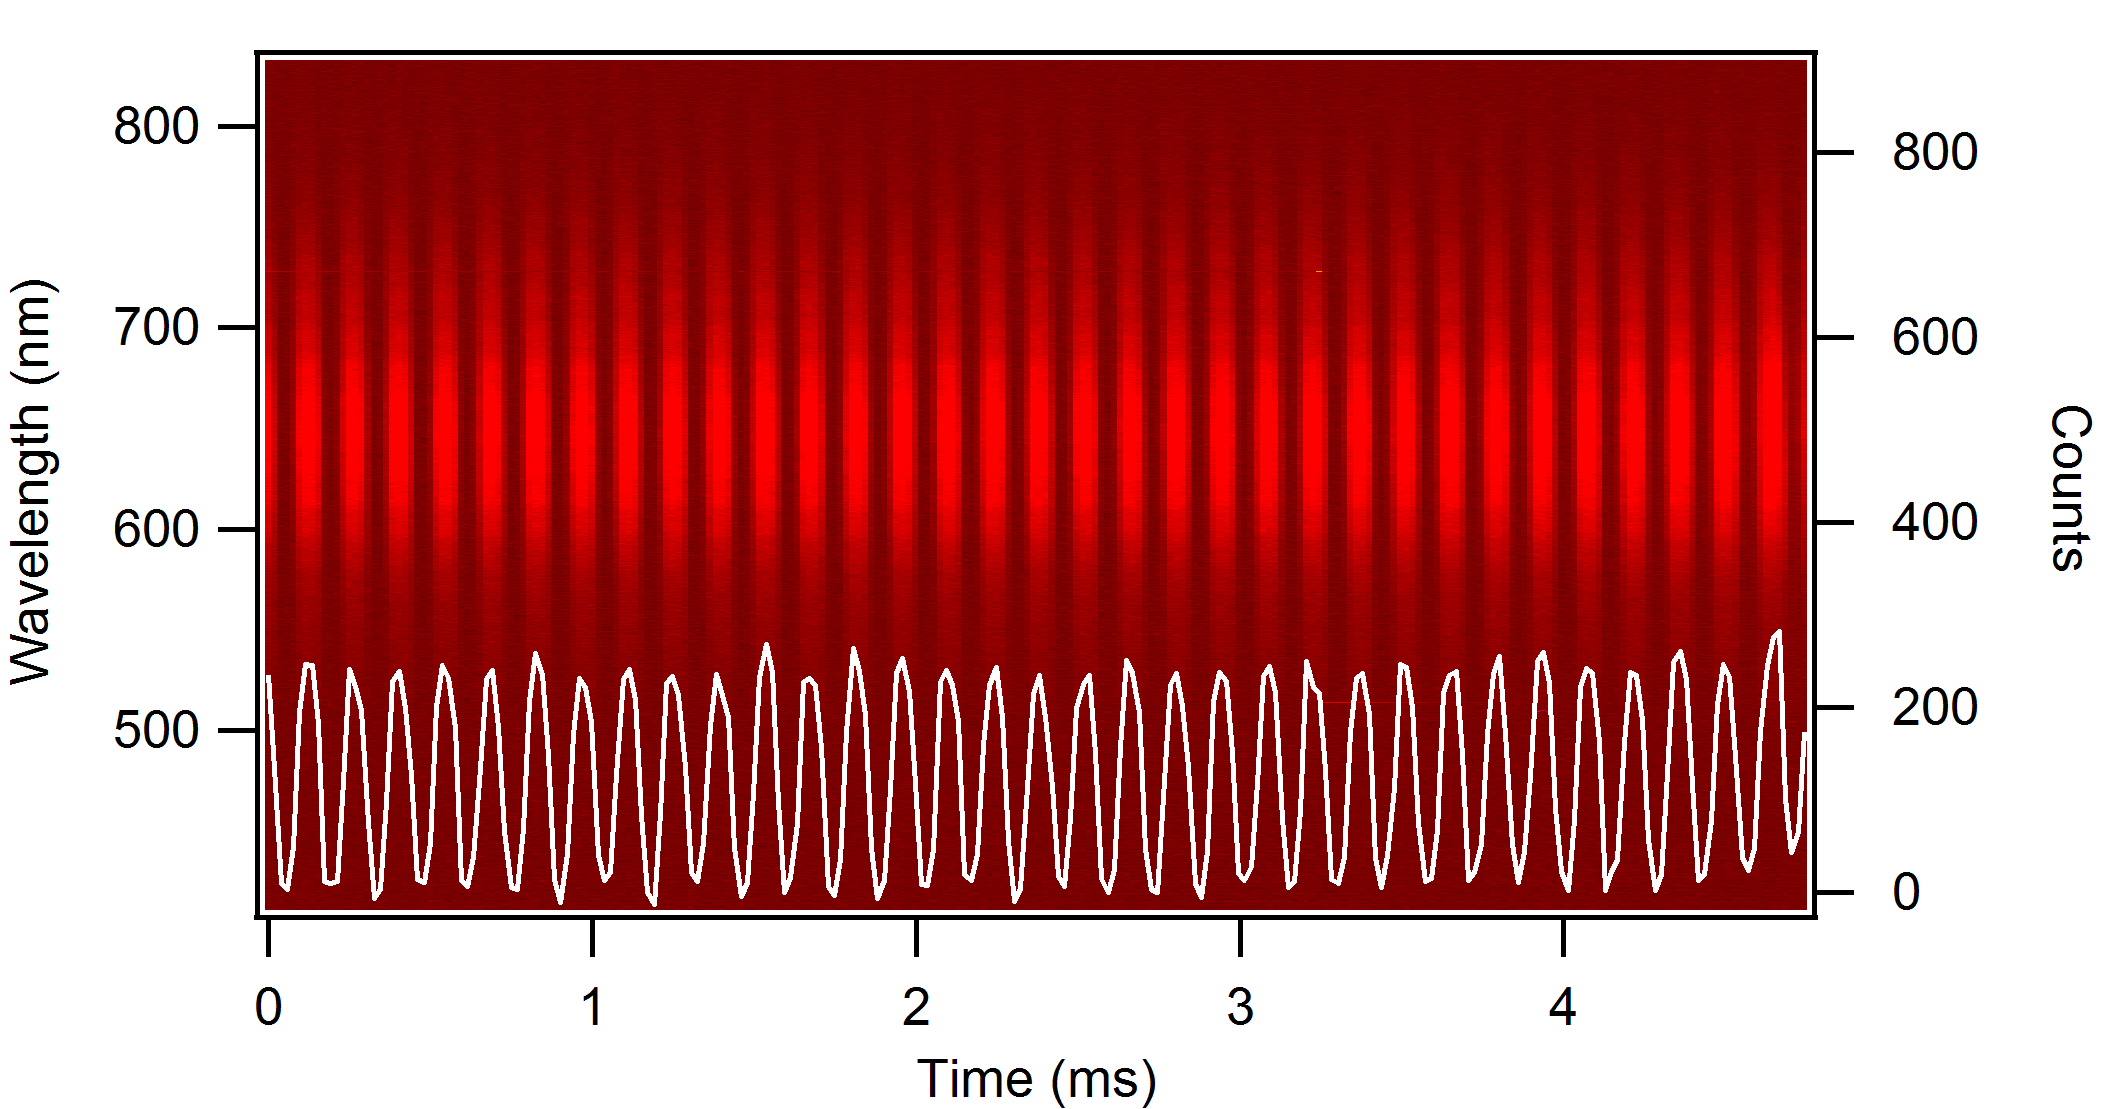
\includegraphics{figures/kinetics_test}
\caption[Testing of kinetics mode acquisition]{\textbf{Testing of kinetics mode acquisition.} A reflected supercontinuum beam is chopped and measured both with kinetics mode on the CCD and by a photodiode on the oscilloscope. Oscillations in the beam at the chopping frequency are clearly seen in both the spectral image and the superimposed photodiode output over a \SI{5}{ms} time period.}
\label{fig:kinetics_test}
\end{figure}

Both make and break contact events typically last no more than \SI{10}{ms} in the current system, often occurring more on a \SI{100}{\micro\second}--\SI{1}{ms} time scale. The kinetics mode has a minimum acquisition time of \SI{2.56}{ms} with a maximum \SI{10}{\micro\second} single spectrum time resolution set by the pixel shift time. The system is trialled using a reflected supercontinuum laser beam with an additional \SI{10}{\micro\second} exposure per row of pixels to give a \SI{5}{ms} measurement, shown in \autoref{fig:kinetics_test}. The beam is chopped and measured on a photodiode to show the system is working as expected. Similar tests were performed with an electronically modulated diode laser to determine the time resolution of measurements.

\begin{figure}[bt]
\centering
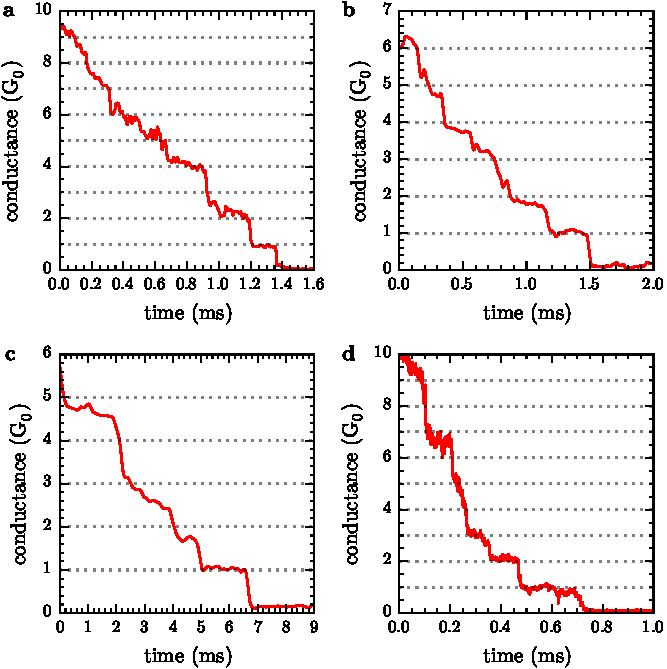
\includegraphics{figures/conductance_traces}
\caption[Examples of fast conductance measurements on tip dimers]{\textbf{Examples of fast conductance measurements on tip dimer break junctions.} During the break the contact conductance drops in units of \G0 until the last atom-atom contact breaks and tips separate.}
\label{fig:conductance_trace}
\end{figure}

\autoref{fig:conductance_trace} shows an example of a conductance traced measured on a break junction between two tips. The traces shows that as the tip contact breaks, the conductance drops in units of \G0. Under these circumstances the CTP modes sustained by the tip dimer are expected to undergo a redshift with decreasing conductance (ideally in discrete quantised steps). Make junctions, as opposed to break junctions, showed more success in tips since the jump into contact is generally a single high quality event whereas in break junctions the forces holding the tip together and the flexibility of the cantilevers causes issues. Tips often exhibit multiple breaks or changes in conductance as the junction vibrates with the final break occurring only once the gap adhesion forces are overcome. Given the strength of the average tip adhesion (and that it often causes the ball to break from the tip apex) the large amount of pulling force applied to the cantilever leads to a very quick sub-\si{\micro\second} break event. This is not possible to measure in the given system. Although the make contact event is typically higher quality it is far more difficult to trigger due to operating near the noise floor, often meaning that the 1\G0 level is too low to reliably observe.

\begin{figure}[bt]
\centering
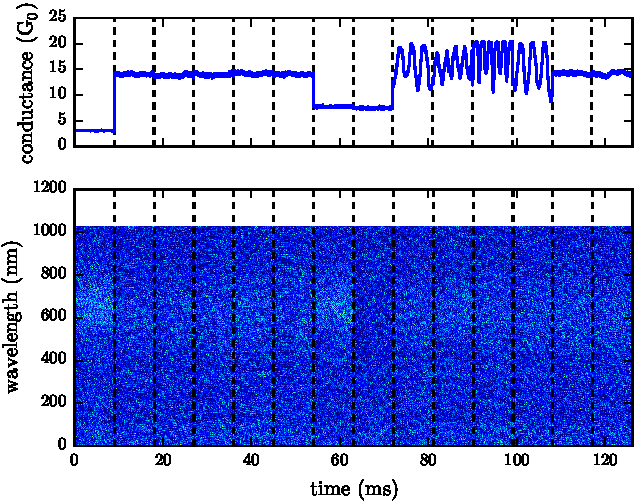
\includegraphics{figures/example_fast_scan}
\caption[]{\textbf{A representative fast scanning measurement from a plasmonic tip dimer.} No signal is detectable with such small exposures per spectrum at acceptable power levels.}
\label{fig:example_fast_scan}
\end{figure}

Though the fast spectroscopy system was engaged in every scan the method provided no useable results. Spectral images contained no detectable signals, as shown in \autoref{fig:example_fast_scan}, due to the short exposure times and low supercontinuum laser powers used to prevent damage to tips. Eventually the \G0-level conductance data was measured using a slow, controlled make junction in a standard spatial scan (shown in \autoref{fig:spherical_tip_scans}b). For this technique to become useful the length of the break or make contact event needs to be lengthened in order to increase the exposure time per row of pixels on the CCD. This could be achieved through more control of the tip position, i.e.\ by using stiff tips in a low humidity environment to minimise adhesion and more controllably break the contact without significantly bending the cantilever. Alternatively, the increased robustness of the electrochemically fabricated plasmonic tips means increased focal intensities could be sustained. By leveraging both of these suggestions in the future, plasmonic MCBJs could be realised as a means of studying conductance at optical frequencies.

\end{document}